\section{Event Selection and Corrections}
  The ideal way to extract an experimental cross section is to use the scattered electrons with the same values of $E_{0}$, $E'$ and $\theta$. However, although the beam energy can be easily locked at one value, $E'$ and $\theta$ can vary within the acceptance of the spectrometer, and due to the statistical limitation, the cross sections can only be calculated by allowing the values of $E'$ and $\theta$ to change within finite ranges, e.g. $\Delta E'$ and $\Delta\Omega$ in Eq.~\eqref{eqxs_org}. In practice, the experimental data is divided by binning one or more kinematic variables with known bin sizes, and the cross section is evaluated at the center of each bin. The way to choose the binning method, including the acceptance ranges and the bin sizes, requires additional corrections during the cross section extraction.
   
   For the E08-014, the data was binned in $E'$ only, and the cross sections were calculated in each $E'$ bin with the same scattering angle, $\theta=\theta_{0}$. The determination of the kinematic space, the acceptance correction and the binning correction will be discussed in this section. A list of cuts to select the good electron events is also given.  
  
\subsection{Central Momentum and Angle}
\begin{figure}[!ht]
  \begin{center}
    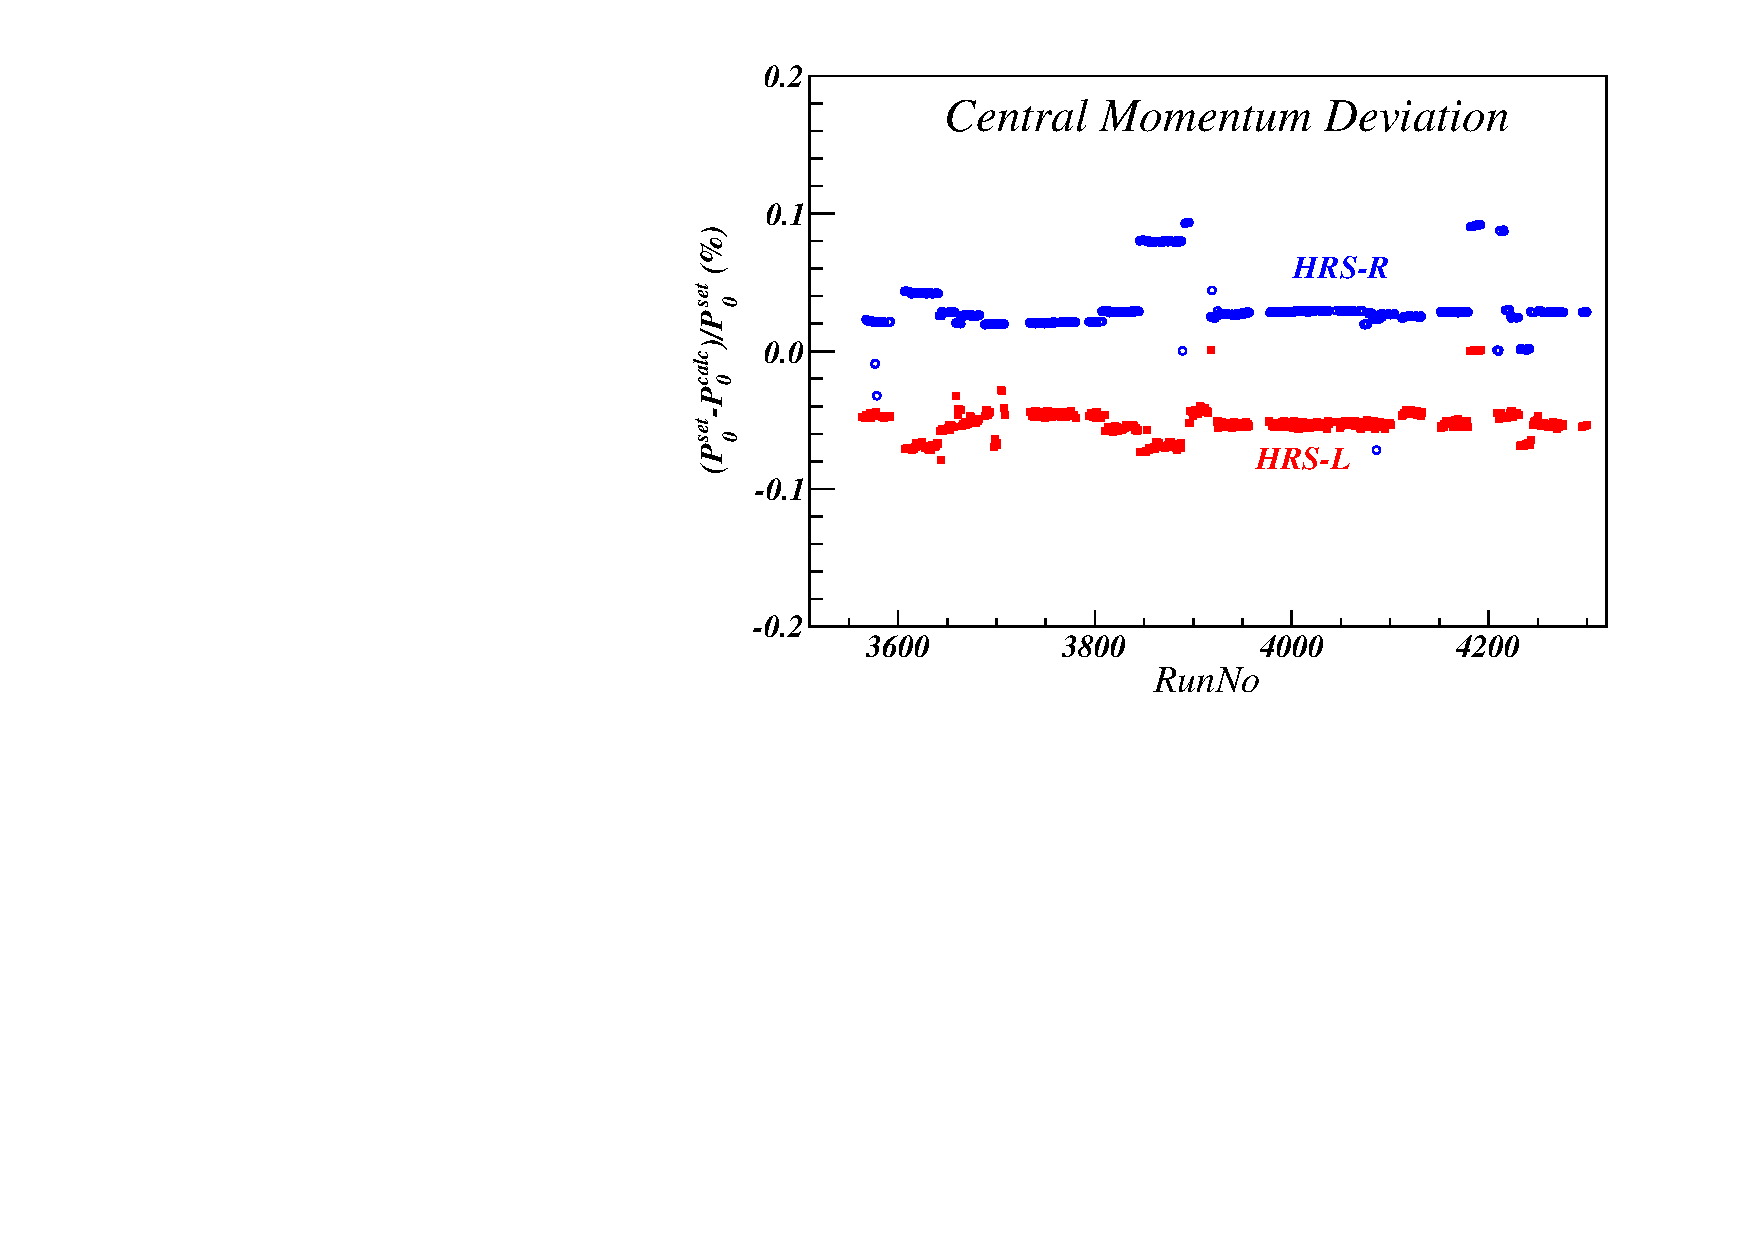
\includegraphics[type=pdf, ext=.pdf,read=.pdf,width=0.60\textwidth]{./figures/xs/point_mom}
    \caption[Central momentum deviation]{\footnotesize{Central momentum deviation, where the blue circles and the red boxes are the deviations of the central momentum on HRS-R and HRS-L, respectively. The x-axis is the run number and the y-axis is the deviation in percentage.}}
    \label{point_mom}
  \end{center}
\end{figure}
The kinematic space is determined by the central scattered momentum, the central scattering angle, and the acceptance of the HRS. The central momentum was given by the field values of the HRS magnets which were locked at the setting values by the HRS NMR system during the experiment. The off-line calculation gives the absolute value of the central momentum with the magnetic field of the dipole~\cite{halla_nim}:
\begin{equation}
 P_{0} = \sum_{i=0}^{4} \gamma_{i} \cdot \left( 10\cdot B^{NMR}_{dipole} \right)^{i},
\end{equation}
where $\mathrm{\gamma_{1,2,3,4}=(0, 270.2, 0, -0.0016)}$ for HRS-L and  $\mathrm{\gamma_{1,2,3,4}=(0, 269.8, 0, -0.0016)}$ for HRS-R. $B^{NMR}_{dipole}$ is the field reading from the NMR monitor. Fig.~\ref{point_mom} shows that the actual central momenta were mostly off by $\pm$3\% while few of them were off by $\pm$10\%. During the cross section extraction, the central momenta were assigned to the calculated values instead of the set values.

The central scattering angle was specified during the experiment by moving the HRS to point at the angle marked on the floor. These floor marks were drawn with respect to the hall center and may not accurately reflect the true values. Moreover, the actual central scattering angle also depends on the offsets between the spectrometer center and the hall center which are different when the spectrometer points at different angles. For some extreme cases, when the spectrometer is moved away from one angle and later moved back to the same value, the actual angles may be different between these two periods.
\begin{table}[!ht]
  \centering
  \begin{tabular}{|c||cccc|}
    \hline
    \textbf{RunNo} &$\theta^{set}_{0}(L)$&$\theta^{true}_{0}(L)$&$\theta^{set}_{0}(R)$&$\theta^{true}_{0}(R)$\\
    \hline \hline
    3565$\sim$3656          & 25.00 & 25.00  & 25.00 & 25.00 \\
    \hline
    3657$\sim$3683          & 21.00 & 21.03  & 21.00 & 21.04 \\
    \hline
     3684$\sim$3708         & 23.00 & 23.00  & 23.00 & 23.01 \\
    \hline
     3735$\sim$3891         & 25.00 & 24.99  & 25.00 & 25.00 \\
    \hline
     3892$\sim$3916         & --    &  --    & 21.00 & 21.03 \\
    \hline
     3917$\sim$4071         & 28.00 & 27.98  & 28.00 & 27.99 \\
    \hline
    4073$\sim$4103          & 21.00 & 21.04  & 28.00 & 27.99 \\
    \hline
    4112$\sim$4179          & 23.00 & 23.00  & 23.00 & 23.04 \\
    \hline
    4181$\sim$4241          & 25.00 & 24.98  & 25.00 & 25.00 \\
    \hline
    4242$\sim$4250          & 21.00 & 21.02  & 21.00 & 21.03 \\
    \hline    
    4251$\sim$4299          & 28.00 & 27.98  & 28.00 & 27.99 \\
    \hline
    \end{tabular}
  \caption{Scattering angle correction}
  \label{scat_angle_table}	
\end{table}

 To obtain the actual central scattering angle each time after the spectrometer was moved, a survey would be performed to correct the errors of the floor marks and to measure the offset between the two centers. Unfortunately, the survey could not been done each time the spectrometers were moved. However, the optics target was surveyed at the beginning of this experiment when both HRSs were set at $\mathrm{25^{\circ}}$, and the positions of $z_{react}$ at different angles can be extracted from the data. Combined with the survey reports from earlier experiments which had similar settings, the actual central scattering angles can be calculated with the difference of $z_{react}$ at $\mathrm{25^{\circ}}$ and at the setting angle ($\Delta z_{react}=z_{react}(\theta_{0})-z_{react}(25^{\circ})$), as follow: 
\begin{eqnarray}
 & &\theta_{tg} = \frac{D_{x}+x_{sieve}-y_{beam}}{L-x_{beam} \cdot sin\theta^{set}_{0}-\Delta z_{react} \cdot cos\theta^{set}_{0}},\\
 & &\phi_{tg}   = \frac{D_{y}+y_{sieve}-x_{beam} \cdot cos\theta^{set}_{0}+\Delta z_{react} \cdot sin\theta^{set}_{0}}{L-x_{beam} \cdot sin\theta^{set}_{0}-\Delta z_{react} \cdot cos\theta^{set}_{0}},\\
 & &\theta^{true}_{0} = acos\left( \frac{cos\theta^{set}_{0}-\phi_{tg}sin\theta^{set}_{0}}{\sqrt{1+\theta_{tg}^{2}+\phi_{tg}^{2}}} \right),
\end{eqnarray}
where $D_{x}$, $D_{y}$, $x_{sieve}$, $y_{sieve}$ and L are given in Table~\ref{optics_offset_table} and Table~\ref{sieve_offset_table}. The beam position ($x_{beam}$, $y_{beam}$) was locked at (-2.668 mm, 3.022 mm) during the experiment. $\theta^{set}_{0}$ is the central scattering reading from the floor marks and $\theta^{true}_{0}$ is the actual central scattering angle after the correction. As shown in Table~\ref{scat_angle_table}, the calculation showed that the maximum offset between $\theta^{true}_{0}$ and $\theta^{set}_{0}$ was not larger than $\mathrm{0.04^{o}}$. The value of $\theta^{true}_{0}$ was calculated for runs taken at each run period when the spectrometer was moved to different positions. The cross sections were calculated with these updated values.

\subsection{Acceptance Correction}
\begin{figure}[!ht]
  \begin{center}
    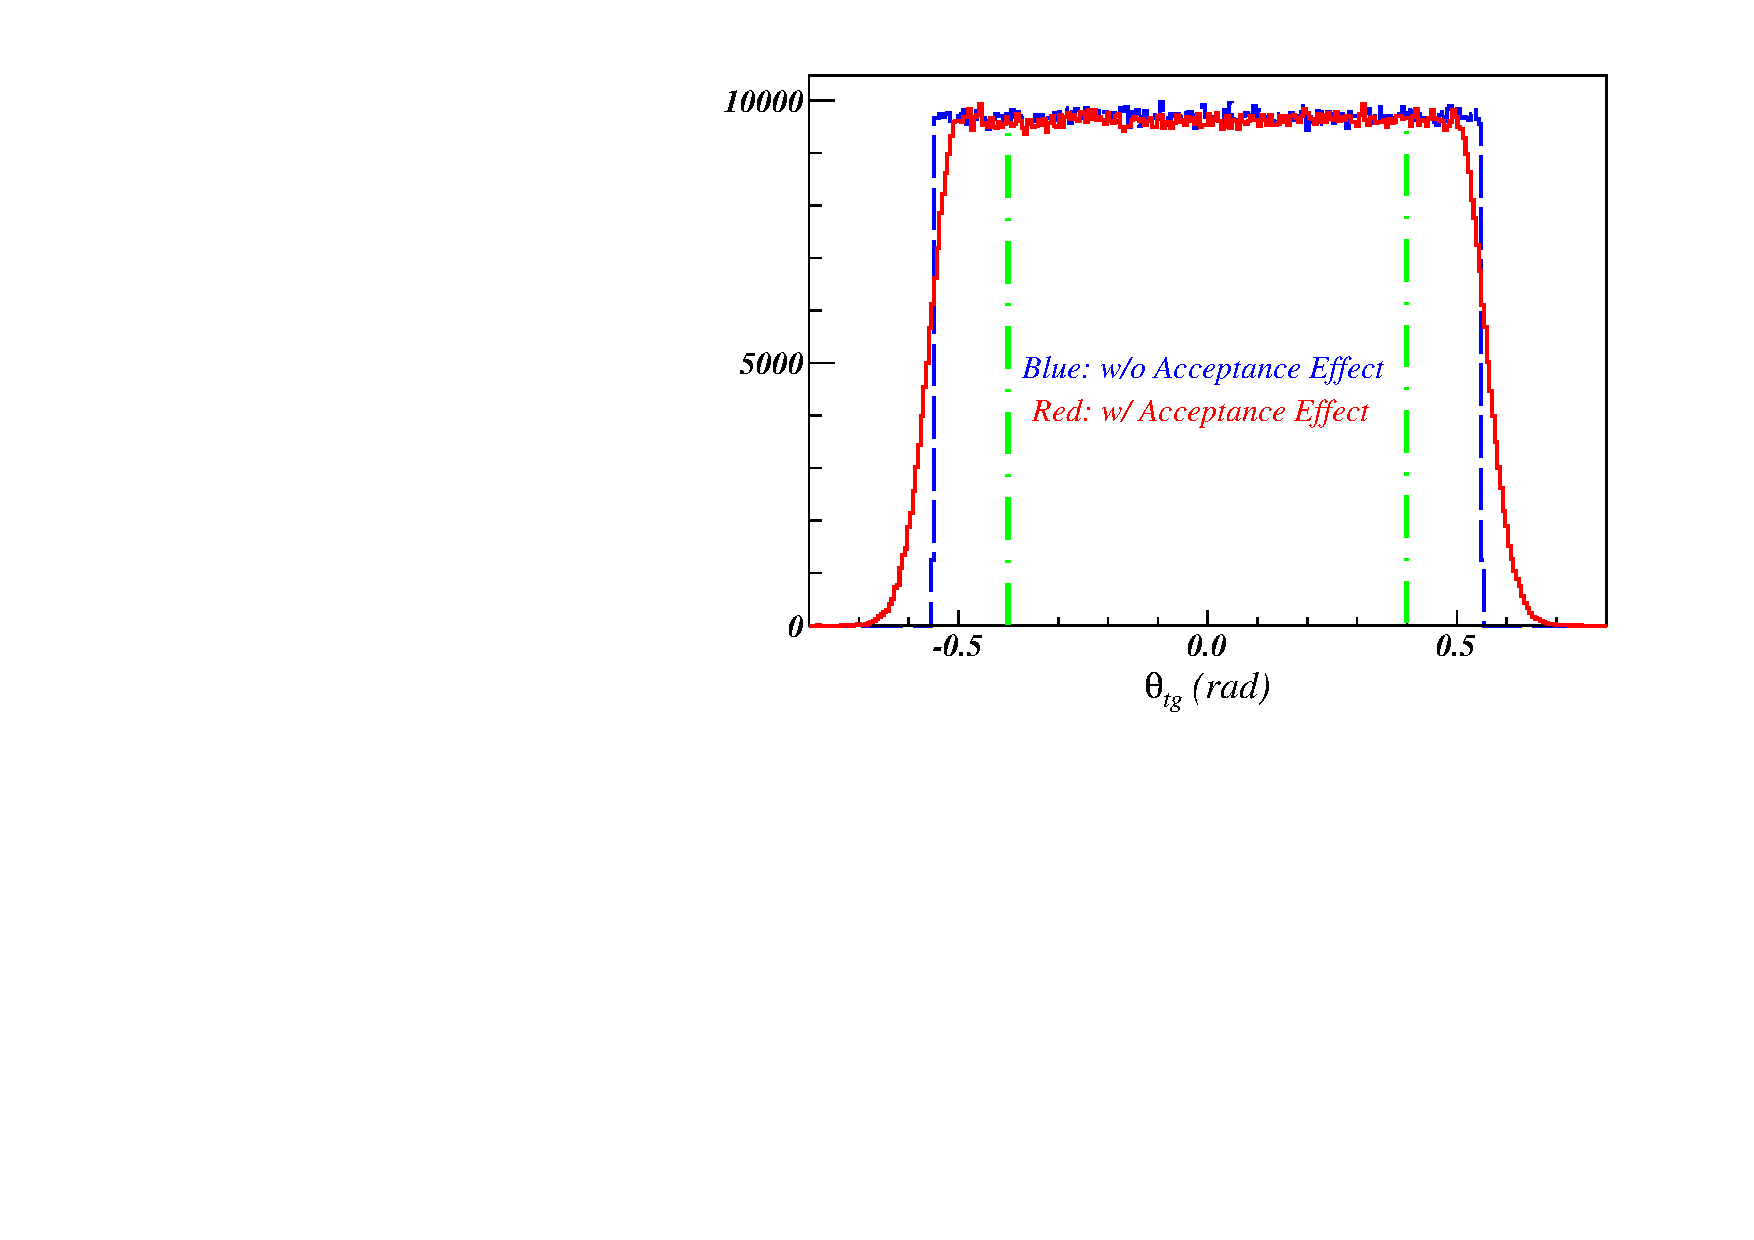
\includegraphics[type=pdf, ext=.pdf,read=.pdf,width=0.60\textwidth]{./figures/xs/accep_demo}
    \caption[A demonstration of the acceptance effect]{\footnotesize{A demonstration of the acceptance effect, where the distribution of $\theta_{tg}$ is generated by assuming no cross section weighting effect. The blue line shows that the acceptance is flat when the HRS acceptance is perfect, while the red line demonstrates the slow fall-off of the acceptance edges. Such an effect is mainly due to the geometry of the HRS magnets and also contributed by the resolutions of the VDC tracking and the optics reconstruction. Green lines show the cuts to select the flat acceptance region.}}
    \label{accp_demo}
  \end{center}
\end{figure}
 The HRS acceptance includes both the range of momentum dispersion ($\Delta\delta p$) and the total solid angle which is the product of the out-of-plane angle ($\theta_{tg}$) and the in-plane-angle ($\phi_{tg}$). For an extended target, the optics reconstructed reaction point along the beam direction ($z_{react}$) is also affected by the HRS acceptance. These four quantities, called the target plane quantities, are essential to reconstruct the reaction at the target. Due to the geometry of the HRS magnets, the event distributions of these quantities are not cut off immediately at the edge of the acceptance and instead, they fall off relatively slowly with a gaussian tail, as can be seen in Fig.~\ref{accp_demo}. In addition, the resolution of VDC tracking and the accuracy of the optics reconstruction can also smear the distributions of these quantities. 
 
 Choosing the right acceptance ranges of the target plane quantities is crucial in order to obtain the correct cross section results. Tight cuts on the target plane quantities were used to select events at the central region of the HRS acceptance. Cutting out the tails on the edges of the focal plane variables also removes multi-scattering events produced inside the spectrometer. The acceptance cuts will be enlarged to increase the statistics of events in one bin, until the cross section results start to deviate from the results calculated with tighter cuts.
 
  However, good events can be incorrectly discarded when one applies the combination cuts of the four target plane quantities to define a valid acceptance region. Such an effect can be corrected by the HRS simulation for each bin:
 \begin{equation}
  A(E_{0},E_{i}, \theta_{0}) = \frac{N^{gen}_{MC}}{\Delta E'_{MC} \Delta\Omega_{MC}}/\frac{N^{i}_{MC}}{\Delta E'_{bin} \Delta\Omega_{EX}},
 \label{acc_corr}  
  \end{equation}
where $\Delta E'_{bin}$ is the bin size of $E'$ and is fixed in both the simulated data and experimental data, and $\Delta\Omega_{EX}$ is the selected angular acceptance range for the experimental data. $N^{i}_{MC}$ is the number of simulated events in the $ith$ bin, with the same acceptance cuts used for the experimental events ($N^{i}_{EX}$) in this bin.  $N^{gen}_{MC}$ is the total number of simulated events without any cuts. $\Delta E'_{MC}$ and $\Delta \Omega_{MC}$ define the full momentum and angular acceptance in the simulation, respectively, and they are slightly larger than the HRS acceptance. Overall,  $\frac{N^{i}_{MC}}{\Delta E'_{bin} \Delta\Omega_{EX}}$ denotes the average number of events in the unit kinematic space which is limited by the HRS geometry, while the other term, $\frac{N^{gen}_{MC}}{\Delta E'_{MC} \Delta\Omega_{MC}}$, gives the average number of events in the unit kinematic space without any spectrometer limitations. Eq.~\eqref{acc_corr} is usually referred to as the acceptance correction. 

\subsection{Binning Correction}
 The cross section results were calculated by binning the data on $E'$. The binning ranges and step sizes are given in the following table:
\begin{table}[!ht]
  \centering
  \begin{tabular}{|c||ccccccccc|}
    \hline
    \textbf{Kin}        & 3.1 & 3.2 & 4.1 & 4.2 &5.0 &5.05 & 5.1 & 5.2 & 6.5 \\
    \hline \hline
    $E'^{Min}$    & 2.76   & 2.90   & 2.71   & 2.88   &2.38   & 2.52   & 2.66   & 2.85   & 2.70   \\
    \hline
    $E'^{Max}$    & 3.05   & 3.21   & 3.00   & 3.19   &2.63   & 2.78   & 2.94   & 3.14   & 2.99   \\
    \hline
    $\Delta E'$      & 0.01   & 0.01   & 0.01   & 0.01   & 0.01  &0.01    & 0.01   & 0.01   & 0.01  \\
    \hline
  \end{tabular}
  \caption{E' binning size and range}
  \label{bin_table}	
\end{table}

  From Eq.~\eqref{eqxs_org}, when binning on $E'$, the cross section in each bin is given as a function of the central scattering angle ($\theta_{0}$) and the momentum value at the center of the bin ($E'_{i}$). However, events in each bin carry different momenta varying from $E'_{i}-\frac{1}{2}\Delta E'$ to $E'_{i}+\frac{1}{2}\Delta E'$ , while their central scattering angles can deviate from $\theta_{0}$ within the solid angle, $\Delta \Omega_{EX}$. A bin-centering correction is applied to remove the effect with the simulation data and the cross section model:
\begin{equation}
 B(E_{0},E_{i}, \theta_{0}) = \frac{\sigma^{rad}_{XEMC}(E_{0},E'_{i},\theta_{0})}{\sum_{j\in i}\sigma^{rad}_{XEMC}(E_{0},E'_{j},\theta_{j})},
  \label{bin_corr}  
\end{equation}
where $\sum_{j\in i}$ means summation over the radiated cross section values, $\sigma(E'_{j},\theta_{j})$), of all Monte Carlo events in the $ith$ bin. $\sigma^{rad}_{XEMC}(E'_{i},\theta_{0})$ and $\sigma^{rad}_{XEMC}(E'_{j},\theta_{j})$ are calculated from the XEMC model.

\subsection{Cuts}
In addition to cutting on the binning variable, there are several other cuts which were applied to select good scattered electron events:
\begin{enumerate}
\item Cutting on production trigger events (see Appendix A);
\item Removing pulser events generated by EDTM modules;
\item Beam trip cut;
\item Selecting events with only one track in VDCs; 
\item Cuts on the focal plane acceptance;
\item Cuts on the target plane acceptance;
\item PID cuts on the GC and the calorimeter.
\end{enumerate}

 When the extraction of cross sections involves data from more than one run, the total number of events after the cuts defined above is given by:
\begin{equation}
  N_{EX}^{i} = \sum_{r} \frac{PS1(3)^{r}\cdot N_{T_{1(3)}}^{r}}{LT_{T_{1(3)}}^{r}},
  \label{eq_nex}
\end{equation}
where $r$ represents the run number and $N_{T_{1(3)}}^{r}$ is the total number of events from $T_{1}$ on HRS-R ($T_{3}$ on HRS-L) and recorded by DAQ after cutting out the beam trip. Note that events from each run are individually corrected by the Live-Time ($LT_{T_{1(3)}}^{r}$) before they are added together.

\section{From Yields to Cross Sections}
The experimental Born cross section can be calculated from Eq.~\eqref{eqxs_org} after applying the acceptance correction (Eq.~\eqref{acc_corr}) and the bin-centering correction (Eq.~\eqref{bin_corr}): 
\begin{equation}
  \sigma^{Born}_{EX} (E'_{i}, \theta_{0}) =  A(E'_{i}, \theta_{0}) \cdot B(E'_{i}, \theta_{0})  \cdot \sigma^{rad}_{EX} (E'_{i}, \theta_{0}) \cdot RC(E'_{i}, \theta_{0}).
  \label{eqxs_org_corr}
\end{equation}
Note that the initial electron energy, $E_{0}$, is fixed at 3.356 GeV during this experiment so it is omitted from the equation. The last term is the radiative correction factor:
\begin{equation}
 RC(E'_{i}, \theta_{0}) = \frac{\sigma^{Born}_{XEMC}(E'_{i},\theta_{0})}{\sigma^{rad}_{XEMC}(E'_{i}, \theta_{0})}.
 \label{eq_radc_fact}
\end{equation}

 Extraction of cross sections from Eq.~\ref{eqxs_org_corr} largely relies on the performance of the simulation and the cross section model, which, however, can not be directly examined from the cross section results. Two useful quantities, the experimental yield and the Monte Carlo (MC) yield, can be extracted to directly compare their differences. The experimental yield is written as:
\begin{equation}
  Y^{i}_{EX} = \frac{N^{i}_{EX}}{N_{e} \cdot \epsilon_{eff}},
  \label{eqyex}
\end{equation}
where $\epsilon_{eff}=\epsilon_{trig}\cdot\epsilon_{vdc}\cdot\epsilon_{e\_cut}^{GC}\cdot\epsilon_{e\_cut}^{calo}$ which are given in Eq.~\eqref{trigger_eff3}, Eq.~\eqref{eq_vdc_eff} and Eq.~\eqref{cut_eff_e}, respectively. The MC yield is given by:
\begin{equation}
  Y^{i}_{MC} = \eta_{tg}\cdot \sum_{j\in i}\sigma^{rad}_{model}(E'_{j},\theta_{j}) \cdot \frac{\Delta\Omega_{MC} \Delta E'_{MC}}{N_{MC}^{gen}}.
  \label{eqymc}
\end{equation}

 The ratio of the experimental yield to the MC yield should be close to one if the performance of the HRS can be well simulated by the MC data and the XEMC model produces cross sections close to the actual values. The experimental Born cross section from Eq.~\ref{eqxs_org_corr} can be rewritten as:
\begin{equation}
  \sigma^{Born}_{EX}(E'_{i}, \theta_{0}) = \frac{ Y^{i}_{EX}}{Y^{i}_{MC}} \cdot \sigma^{Born}_{XEMC}(E'_{i}, \theta_{0}),
  \label{eqxs_ratio}
\end{equation}

The yield ratio method can largely reduce the bias caused by the choice of different cross section models and Monte Carlo simulation tools. While the experimental yield is completely extracted from the data and remains unchanged, one can iterate the cross section model and apply necessary corrections only on the MC yield until the the yield ratio becomes close to one for all $E'$ bins. Furthermore, the acceptance cuts on the HRS can also be studied by varying the cuts and checking the distribution of the yield ratio as a function of the binning variable. Most of other potential issues, such as junk runs, incorrect input parameters and so on, can also be examined in the yield ratio method.

%\subsection{Comparing Yields.}
%  Fig.~\ref{ld2_yield} through Fig.~\ref{ca48_yield} show the distribution of the yields and the yield ratio for all targets used in this experiment. From the ratio plots, the experimental yield and the MC yield agree nicely 

\section{Calculation of Errors}
 One of the most important tasks in the extraction of experimental cross sections is to calculate the systematic errors and statistical errors. Systematic errors are introduced by the experimental instrumentation, the simulation tools and the cross section model, etc. Statistical errors are related to the number of measurements of one quantity during the experiment. It is very important to properly propagate the errors when extracting new quantities from the existing quantities, and any mistakes such as mis-counting or double-counting should be avoided during the cross section extraction. The detailed explanation of the error calculation and propagation is given in the following subsections.

\subsection{Statistical Errors}
 A detailed propagation of statistical errors is discussed here:
\begin{enumerate}

\item \textbf{$N_{e}$:} From Eq.\ref{eq_ne}, since the charge is obtained from the average of two BCM monitor outputs ($U_{1}$ and $D_{1}$),the error is also averaged:
  \begin{equation}
   \delta N_{e}^{r} = \sqrt{\frac{\left(\delta N_{e}^{r,D_{1}}\right)^{2}+\left(\delta N_{e}^{r,U_{1}}\right)^{2}}{2}}
                    = \sqrt{\frac{N_{e}^{r,D_{1}}+N_{e}^{r,U_{1}}}{2}}
                    = \sqrt{\frac{N_{e}^{r}}{2}},
  \end{equation}
where, $r$ means the run number. Hence,
  \begin{equation}
    \delta N_{e} = \sqrt{\sum_{r}\left(\delta N_{e}^{r}\right)^{2}}=\sqrt{\frac{\sum_{r}N_{e}^{r}}{2}}=\sqrt{\frac{N_{e}}{2}}.
  \end{equation}
  
\item \textbf{Live-Time:} Form Eq.\ref{eq_lt}, when  $PS^{r} = 1$:
  \begin{equation}
    \delta LT^{r} = LT^{r} \cdot \sqrt{\frac{1}{N^{r,Scaler}}+\frac{1}{N^{r,DAQ}}},
  \end{equation}
where $PS=PS1$ for HRS-R and $PS=PS3$ for HRS-L. When  $PS^{r} > 1$, the calculation of $\delta LT^{r}$ is given differently~\cite{vince_thesis}:
 \begin{equation}
   \delta LT^{r} = LT^{r} \cdot \sqrt{\frac{1}{N^{r,Scaler}}-\frac{1}{N^{r,DAQ}}}.
 \end{equation}

\item \textbf{$N_{EX}:$} From  Eq.\ref{eq_nex} and $N_{EX}=\sum_{r}N_{EX}^{r}$ for all runs, one gets:
  \begin{equation}
    \delta N_{EX}^{r} = N_{EX}^{r} \cdot \sqrt{\frac{1}{N_{recorded}^{r}} + \left(\frac{\delta LT^{r}}{LT^{r}}\right)^{2} }, \delta N_{EX}=\sqrt{\sum_{r}\left(\delta N_{EX}^{r}\right)^{2}},
  \end{equation}
where $N_{recorded}^{r}$ is defined in Eq.~\eqref{eq_lt}. 

\item \textbf{$Y_{EX}:$} From Eq.\ref{eqyex},
  \begin{equation}
    \delta Y_{EX} =  Y_{EX} \cdot \sqrt{\left(\frac{\delta N_{EX}}{N_{EX}}\right)^{2}+\left(\frac{\delta N_{e}}{N_{e}}\right)^{2}+\left(\frac{\delta\epsilon_{eff}}{\epsilon_{eff}}\right)^{2}},
  \end{equation}
where $\epsilon_{eff}$ is set to one and its statistic error and systematic error are set to zero and 1\%, respectively.

\item \textbf{$Y_{MC}:$} From Eq.\ref{eqymc},
  \begin{equation}
    \delta Y_{MC} =  Y_{MC} \cdot \sqrt{\left(\frac{\delta\sum_{j\in i}}{\sum_{j\in i}}\right)^{2}+\left(\frac{\delta N_{MC}^{gen}}{N_{MC}^{gen}}\right)^{2}},
  \end{equation}
  where $\delta\sum_{j\in i} = \sum_{j\in i}\cdot\frac{1}{\sqrt{N_{MC}^{i}}}$, since it summarizes the cross section of MC events ($N_{MC}^{i}$) in one bin.

\item \textbf{$\sigma_{EX}^{Born}:$} From Eq.\ref{eqxs_ratio},
  \begin{equation}
    \delta \sigma_{EX}^{Born} = \sigma_{EX}^{Born} \cdot \sqrt{\left(\frac{\delta Y_{EX}}{Y_{EX}}\right)^{2}+\left(\frac{\delta Y_{MC}}{Y_{MC}}\right)^{2}}.
  \end{equation}

\end{enumerate}

\subsection{Systematic Errors}
 The entire list of systematic errors has not been determined in this thesis. Few items are given as follows:
\begin{enumerate}
\item \textbf{$\eta_{tg}$:}  Form Eq.~\eqref{eq_ntg} and Eq.~\eqref{eq_tgrho}, there are three quantities that can introduce errors: beam current measurement and calculation ($\delta I$), accuracy of Boiling Factors ($\delta B$), and the accuracy of target thickness measurement ($\delta \rho$). First two terms were temporarily set to zero, hence:
  \begin{equation}
    \delta \eta_{tg} = \frac{\delta\rho}{\rho} \cdot \eta_{tg}.
  \end{equation} 
The value of $\delta \rho$ for each target can be found in Table~\ref{target_table} and in Ref.~\cite{target_report}.
\item \textbf{$\epsilon_{eff}$:}  1\% systematic errors is assigned to each of VDC One-Track efficiency, trigger efficiency, detection and cut efficiencies of Gas \v{C}erenkov and Calorimeters.
%\item \textbf{Optics:}
\item \textbf{$\delta p$ correction (HRS-R only):} The error caused by correcting the un-calibrated $\delta p$ on HRS-R as given in Appendix D has to be evaluated. 0.3\% is assigned in this thesis. The value will be updated in the near future.
\item \textbf{Cross section model and radiative correction:} The error from the cross section models and the radiative correction. An estimation of 3\% is given in this thesis. The value will be updated in the near future.
\end{enumerate}